% =============================================================================
% FILE NAME : 02_related_work.tex
% DEPARTMENT: University of Tuebingen
% AUTOR     : Tom Schammo
% =============================================================================
% CONTENT   : Include for chapter "Related Work"
% =============================================================================

\section{Rust on the PULPissimo}

The code in this thesis is built upon the foundations built by Raphael Vogelgsang in his thesis \emph{'Rust auf der RISCV Plattform PULPissimo – Entwicklung und
Evaluation'} \cite{rust_pulp}.
He built the Peripheral Access Crate (PAC) and Hardware Abstraction Layer (HAL) which I use and extend to add support for the UltraTrail architecture.
The PAC provides direct access to peripherals and has been generated using the '\lstinline{svd2rust}' tool \cite{svd2rust}.
This tool uses a System View Description (SVD) file, which uses the XML format to describe certain properties like registers and peripherals, and are
thereby unique for each microcontroller.
SVD files are usually provided by the vendor, but in this case it had to be written from scratch.
The HAL builds upon the PAC and provides a layer of abstraction between the programmer and the hardware.
It implements a user-friendly API that removes the need for detailed knowledge about the hardware architecture.

\section{Previous work on the PULPissimo}

The chair for embedded systems has developed some C libraries for the PULPissimo that provide drivers and tests.
They serve as an orientation and comparison for the Rust libraries.

\section{UltraTrail}

UltraTrail is a 'configurable ultra-low power TC-ResNet AI accelerator for efficient keyword spotting' \cite{ultratrail}.
It uses temporal convolutional networks (TCNs) combined with residual networks (TC-ResNet) for intelligent sensor signal processing.
They show superior behavior compared to conventional convolutional neural networks (CNNs) and long short-term memory (LSTM) networks,
which is a type of Recurrent Neural Network (RNN), and commonly used speech recognition applications like keyword spotting or text to speech engines.
TCNs specifically not only appear to be more accurate, but also simpler and clearer compared to LSTMs and GRUs \cite[Ch I]{ultratrail}.\\
UltraTrail uses a variety of units, arrays and layers to provide efficient mapping of the TC-ResNet without sacrificing too much flexibility.
An overview of the UltraTrail system architecture can be seen in figure \ref{fig:ultratrail_arch}.

\begin{figure}[htb]
    \centering
    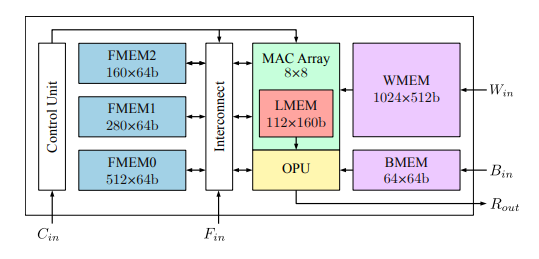
\includegraphics[width=0.9\textwidth]{figures/ultratrail.png}
    \caption[Illustration: The UltraTrail system architecture \cite{ultratrail}]{The UltraTrail system architecture}
    \label{fig:ultratrail_arch}
\end{figure}

\section{Keyword spotting in the Industry}

\subsection{Voice Assistants}

Keyword spotting is mainly used in voice assistants (VAs), like Siri by Apple \cite{siri} or Amazon's Alexa \cite{alexa}.
The devices they run on (like Amazon Echo Dot) use keyword spotting to 'activate', after which they start
to 'actively listen' to perform your command.
There are also open source alternatives to the popular products by the aforementioned tech giants, like Mycroft by \lstinline{mycroft.ai} \cite{mycroft}.
Snips.ai used to be another alternative VA to the products by Apple and Amazon, however, they have been acquired by Sonos in November 2019 \cite{sonos_snips}.
Snips used also used a keyword spotting to 'activate' the VA that the user could then communicate with, however, they also advertise their focus
on privacy and offline, on device speech processing.
However, their product was not open source, so there is limited knowledge available about their system.
They do advertise customizable 'wake words', and mentioned hardware requirement on a snapshot of their website \cite{snips_flow}.
It was possible to run their system on devices like the Raspberry Pi 3 \cite{rpi3} or Jetson TX2 \cite{jetson_tx2},
as well as the Snapdragon 410 \cite{snapdragon_410} by Qualcomm, which had been used in phones like the Samsung Galaxy J5 or Xiaomi Redmi 2.
Since there is not a lot of public knowledge available for proprietary systems like Siri, Alexa or Snips, I will take a more in depth look at Mycroft only.

\subsubsection{Mycroft}

Mycroft is an open source \cite{mycroft_gh} and privacy focused VA \cite{mycroft}.
It runs a variety of devices like the Raspberry Pi, common desktop devices, but also custom hardware, the manufacturer claims.
Like Alexa, Mycroft can be extended by adding skills \cite{mycroft_skills}, which can either be acquired for free on their marketplace,
from GitHub or self-made.\\\\
Mycroft consists of several technologies; 'Mimic' \cite{mycroft_mimic3}, their text-to-speech engine, 'Adapt' \cite{mycroft_adapt} and 'Padatious' \cite{mycroft_padatious},
their intent parsers for natural language understanding, and most interestingly for this thesis, 'Precise' \cite{mycroft_precise} their wake word listener.\\
Precise uses a type of RNN, a Grated Recurrent Unit (GRU), illustrated in \ref{fig:precise_gru}.


\begin{figure}[htb]
    \centering
    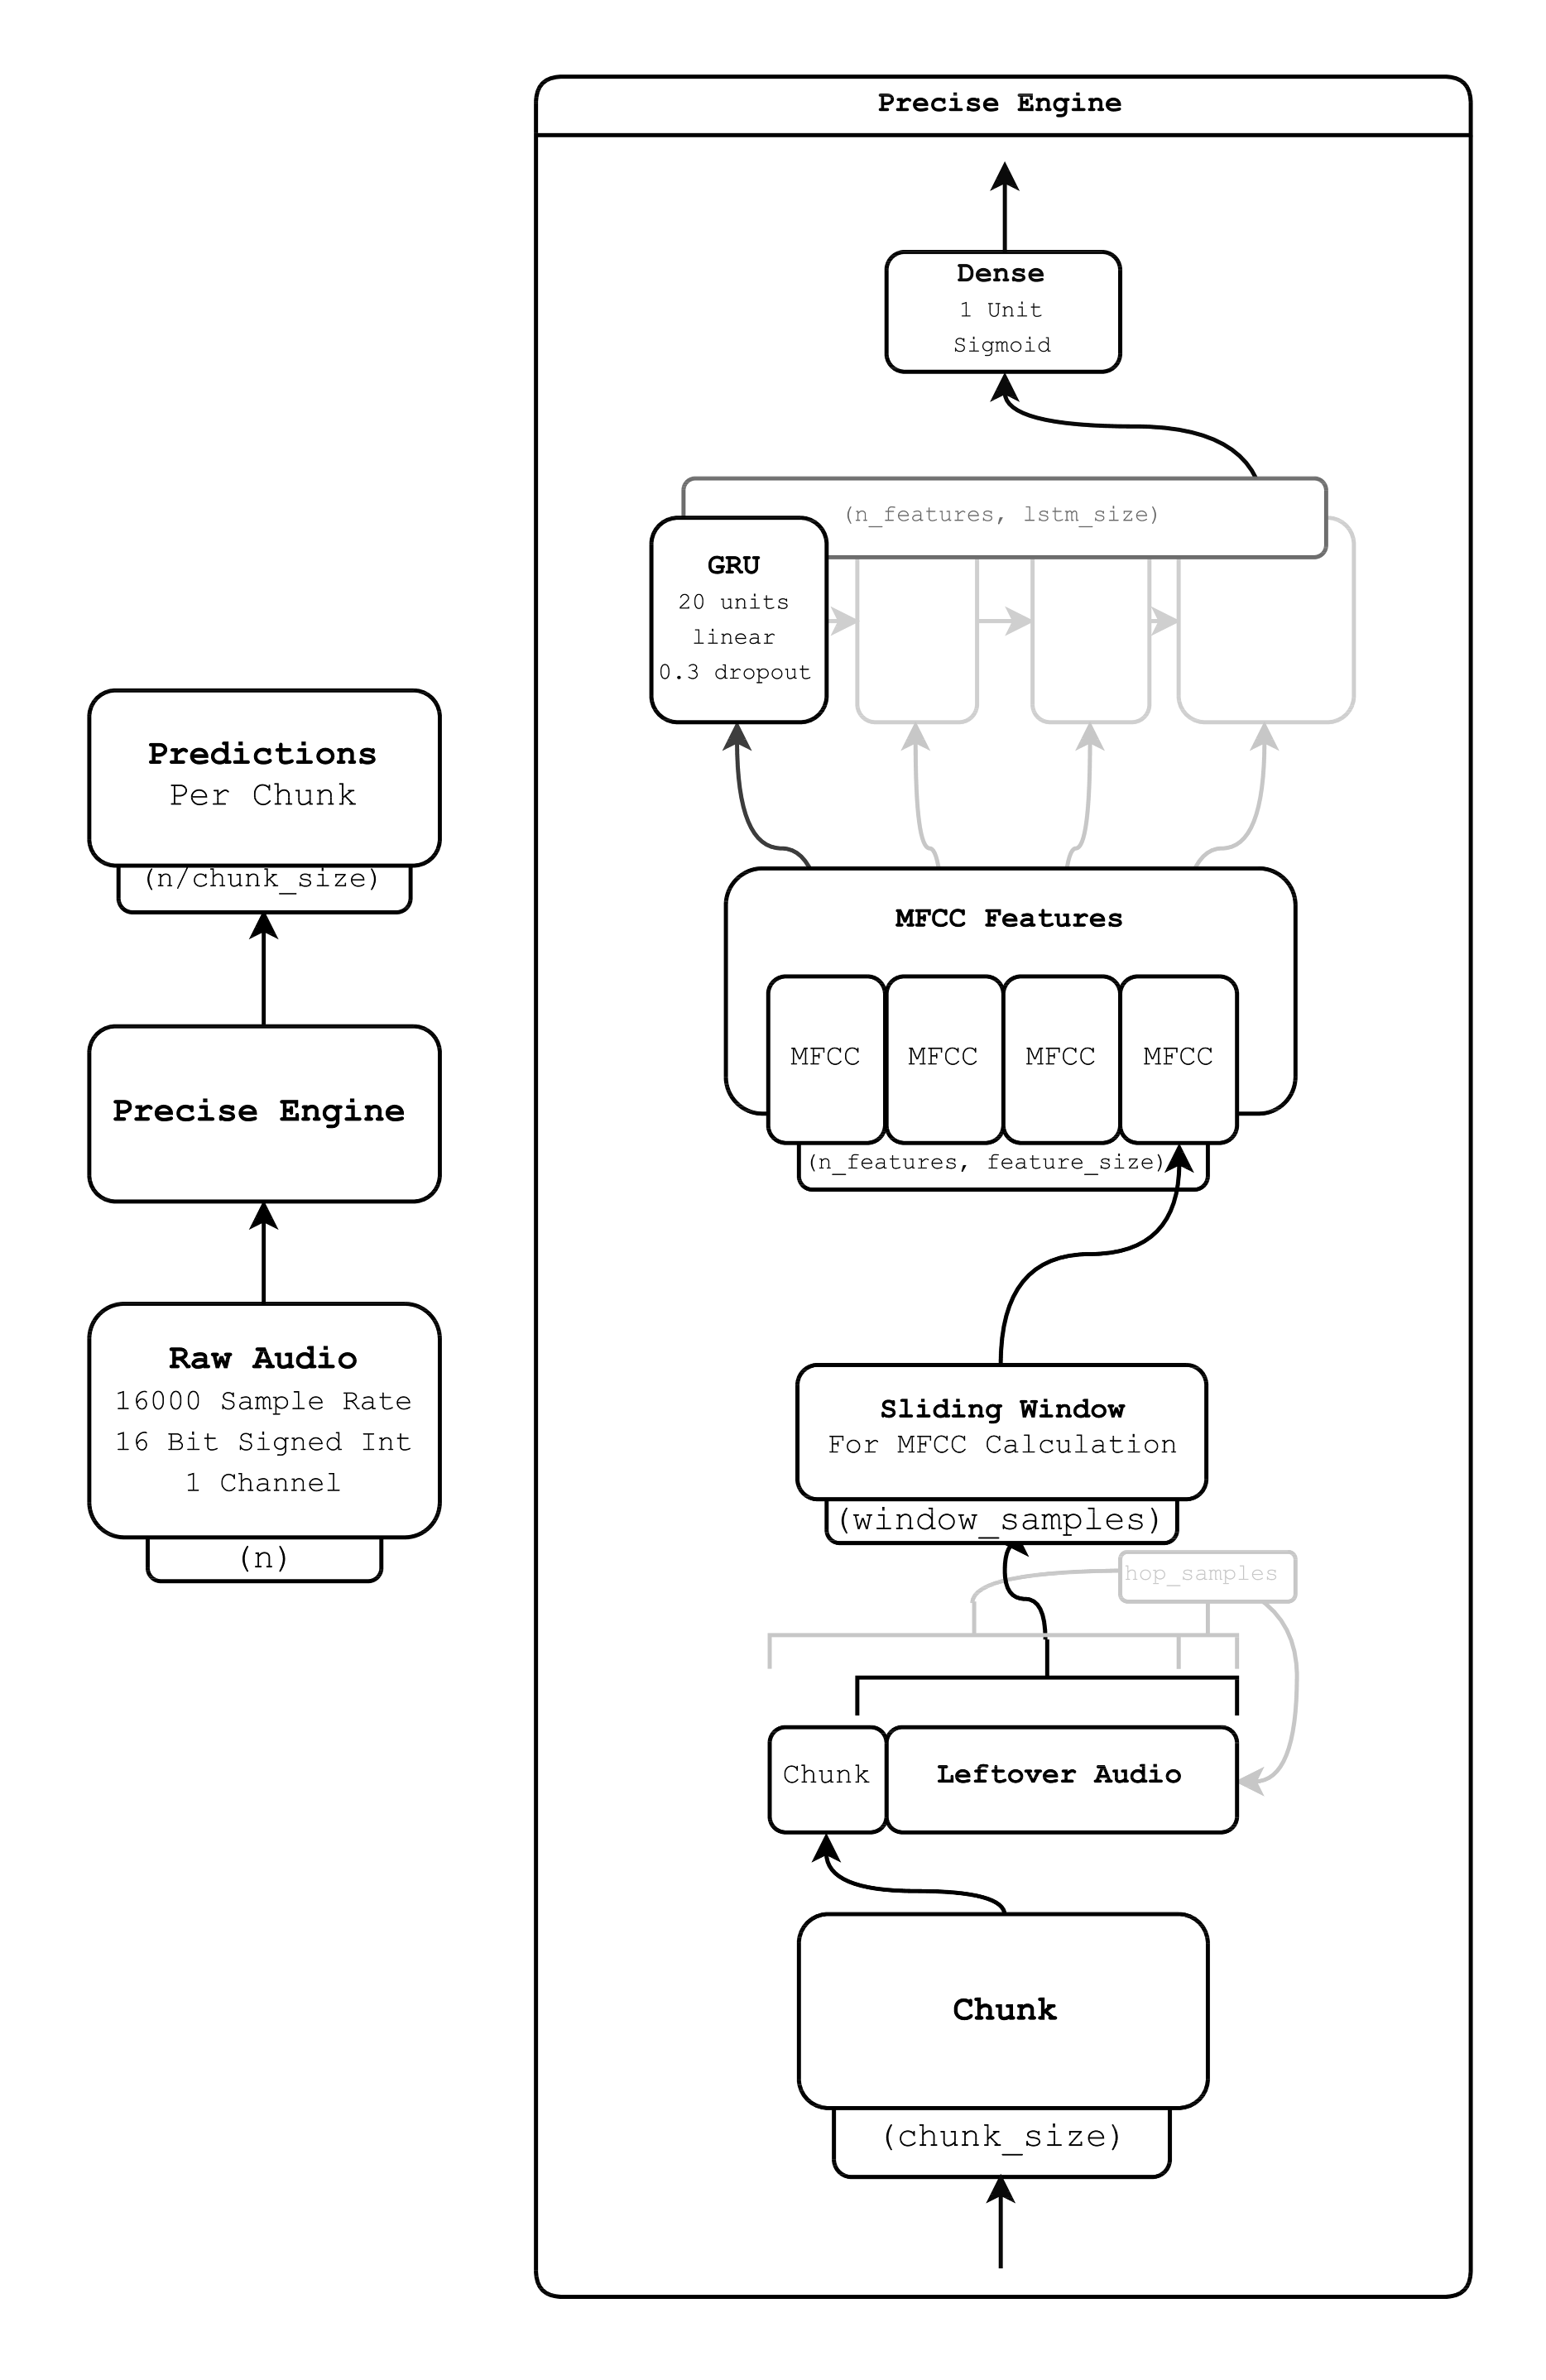
\includegraphics[width=0.9\textwidth]{figures/precise_engine.PNG}
    \caption[Illustration: The 'Precise' engine \cite{mycroft_precise}]{The 'Precise' engine illustrated}
    \label{fig:precise_gru}
\end{figure}


